\documentclass[12pt,a4paper,notitlepage,twoside]{article}
% dans ce modèle article ne pas utiliser la mention "chapter", par contre on peut
% utiliser la numérotation naturelle et les références croisées.
\usepackage[utf8x]{inputenc}
\usepackage{ucs}
\usepackage[french]{babel}
\usepackage[T1]{fontenc}
%\usepackage{eurosym} % pour pouvoir utiliser le symbole \euro{}
\usepackage[left=17mm,right=17mm,top=17mm,bottom=17mm]{geometry}
% définition du nombre de lignes à afficher en fin ou en début de page pour
% éviter les veuves et orphelines.
\usepackage[all, defaultlines=3]{nowidow}
\usepackage{array}
\usepackage[table]{xcolor} % pour couleur de blocs, permis avec \color{couleur}{texte}

\usepackage{multirow}
\usepackage{multicol}
	\setlength{\columnsep}{0.6cm}
	\setlength{\columnseprule}{1pt}
	\def\columnseprulecolor{\color{black}}

%\usepackage{wrapfig}
% \begin{wrapfigure}[lineheight]{position = r R l L i I o O}{width}
%  minuscule = float, majuscule = force emplacement
% \end{wrapfigure}

\usepackage{hyperref} %support des url via le tag \url
\hypersetup{
	colorlinks=true,
	linkcolor=blue,
	urlcolor=purple,
	}
	\urlstyle{same}
\usepackage{amsmath}
\usepackage{amsfonts}
\usepackage{amssymb}

\usepackage{textcomp}

\usepackage{graphicx}
%\graphicspath{ {./Images/} } % indique le chemin relatif où sont situées les images
% définition de la clé Graphic Inclusion pour paramétrer par défaut la taille des images incluses
	\setkeys{Gin}{width=0.7071\linewidth}
\usepackage{float}
	\floatplacement{table}{H} %par défaut tables là où code est posé
	\floatplacement{figure}{H} %par défaut images là où code est posé
\usepackage{siunitx}
	\sisetup{locale = FR}
%%%% Packet circuitikz permet de dessiner des circuits électriques, peut nécessiter l'utiliation de siunitx
%\usepackage[european]{circuitikz}
%\usetikzlibrary{babel}
%\usepackage{qrcode}
%\usepackage{pgfplots} %permet de tracer directement des graphiques depuis latex

\usepackage{ifthen}
%%% Gestion de la dyslexie
\newboolean{isDyslexique}
	\setboolean{isDyslexique}{false}
%%% Gestion de la correction
\newboolean{isCorrection}
	\setboolean{isCorrection}{false}
\newboolean{isEvaluation}
	\setboolean{isEvaluation}{false}

% \usepackage{palatino} %\usepackage{sans}
% \usepackage{lxfonts} %\usepackage{arev}
\ifthenelse{\boolean{isDyslexique}}{% si vrai :
	\usepackage{arev}
	\renewcommand{\baselinestretch}{1.5}
}{% si faux :
	\usepackage{lmodern}
	\renewcommand{\baselinestretch}{1.25}
}
\usepackage{lastpage}
% test de modification des headers et footers
\usepackage{fancyhdr}
\pagestyle{fancy}
\fancyhf{}
\fancyhead[LE,RO]{\rightmark}
\fancyhead[LO,RE]{\leftmark}
\fancyfoot[LE,RO]{F.S.G.}
\fancyfoot[C]{.::--- \ \thepage / \pageref*{LastPage} \ ---::.}
\fancyfoot[RE,LO]{Titre}
% fin du test de modification :)
\usepackage{tikz}
	\usetikzlibrary{babel,math}
% inclusion du paquet bclogo pour boîtes avec logo de mise en exergue
\usepackage[tikz]{bclogo}

% ========= DÉFINITION D'UN INTERLIGNE DIFFÉRENT ===============
\setlength{\parskip}{0.1cm} % définit l'espacement entre paragraphes
\renewcommand{\thesection}{\Roman{section}}

\author{F.G.}
% éviter le titre peut-être ?
\title{}

\begin{document}
%%% CARTOUCHE D'IDENTIFICATION %%%
\begin{flushleft}
\begin{tabular}{| m{0.15\linewidth} m{0.78\linewidth} |}
	\hline
	\multirow{4}{*}{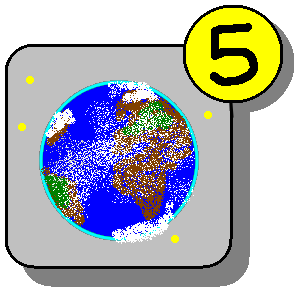
\includegraphics[width=\linewidth]{cycle5-logo-terre.png}}	
	& c5-2.th3.ac2
	\begin{LARGE}
	Se localiser et mesurer avec des coordonnées sphériques.
	\end{LARGE} \\ [0.5ex]
	\cline{2-2}
	 & NOM : . \ . \ . \ . \ . \ . \ . \ . \ . \ . \ . Prénom : . \ . \ . \ . \ . \ . \ . \ . \ . \ . \ . \\
	 & \\
	 & Classe : . \ . \ . \ . Durée : . \ . \ . \ . min. \\ [1ex]
	\hline
\end{tabular}

%%% CARTOUCHE DE NOTATION %%%
\ifthenelse{\boolean{isEvaluation}}{%true
	\begin{flushleft}
		\begin{tabular}{| m{0.15\linewidth} | m{0.8\linewidth} ||}
			\hline
			NOTE : & APPRÉCIATION : \cr
			$ ~~ $ & $ ~~ $ \cr
			$ ~~ $ & $ ~~ $ \cr
			$ ~~ $ & $ ~~ $ \cr
			$ ~~ $ & $ ~~ $ \cr
			$ ~~ $ & $ ~~ $ \cr
			\hline\hline
		\end{tabular}
	\end{flushleft}
}{%false
	\relax
} % fin cartouche ntoation

%%% CARTOUCHE D'ÉVALUATION DES COMPÉTENCES %%%
\begin{tabular}{| m{0.05\linewidth} | m{0.725\linewidth} | m{0.015\linewidth} | m{0.015\linewidth} | m{0.015\linewidth} | m{0.015\linewidth} |}
\hline
\multirow{2}{*}{Réf.} & \multirow{2}{*}{Intitulé Compétences cycle 5} & \multicolumn{4}{c |}{État} \\
\cline{3-6}
	& & I & F & S & T \\
\hline
%Ap 1 & Énoncer une problématique. & & & & \\ \hline
%Ap 2 & Rechercher et organiser l’information en lien avec la problématique étudiée. & & & & \\ \hline
%Ap 3 & Représenter la situation par un schéma. & & & & \\ \hline
%Ra 1 & Formuler des hypothèses. & & & & \\ \hline
%Ra 2 & Proposer une stratégie de résolution. & & & & \\ \hline
%Ra 3 & Planifier des tâches. & & & & \\ \hline
Ra 4 & Évaluer des ordres de grandeur. & & & & \\ \hline
%Ra 5 & Choisir un modèle ou des lois pertinentes. & & & & \\ \hline
%Ra 6 & Choisir, élaborer, justifier un protocole. & & & & \\ \hline
%Ra 7 & Faire des prévisions à l'aide d'un modèle. & & & & \\ \hline
%Ra 8 & Procéder à des analogies. & & & & \\ \hline
%Ré 1 & Mettre en œuvre les étapes d’une démarche. & & & & \\ \hline
%Ré 2 & Utiliser un modèle. & & & & \\ \hline
Ré 3 & Effectuer des procédures courantes (calculs, représentations, collectes de données, etc.). & & & & \\ \hline
%Ré 4 & Mettre en \oe{}uvre un protocole expérimental en respectant les règles de sécurité. & & & & \\ \hline
%Va 1 & Faire preuve d’esprit critique, procéder à des tests de vraisemblance. & & & & \\ \hline
Va 2 & Identifier des sources d’erreur, estimer une incertitude, comparer à une valeur de référence. & & & & \\ \hline
%Va 3 & Confronter un modèle à des résultats expérimentaux. & & & & \\ \hline
Va 4 & Proposer d’éventuelles améliorations de la démarche ou du modèle. & & & & \\ \hline
%Co 1 & présenter une démarche de manière argumentée, synthétique et cohérente. & & & & \\ \hline
%Co 2 & utiliser un vocabulaire adapté et choisir des modes de représentation appropriés & & & & \\ \hline
%Co 3 & échanger entre pairs. & & & & \\ \hline
\end{tabular}

\end{flushleft}

\section*{Points du programme abordés.}
\begin{multicols}{2}
\subsubsection*{Savoirs}
On repère un point à la surface de la Terre par deux coordonnées angulaires, sa latitude et sa longitude.

Le plus court chemin entre deux points à la surface de la Terre est l’arc du grand cercle qui les relie.
\columnbreak

\subsubsection*{Savoir faire}
Calculer la longueur d’un arc de méridien et d’un arc de parallèle.

Comparer, à l’aide d’un système d’information géographique, les longueurs de différents chemins reliant deux points à la surface de la Terre.
\end{multicols}

\section*{Matériel à disposition.}
Chaque groupe d'élèves est équipé d'une tablette ou d'un smartphone et de l'application SatStat.

\section*{Objectif.}
Se familiariser avec les notions de latitude et de longitude, de ma, effectuer des mesures et des calculs de longueur.

\newpage
\vfill
\section*{Plan du lycée.}
\begin{figure}
	\centering
	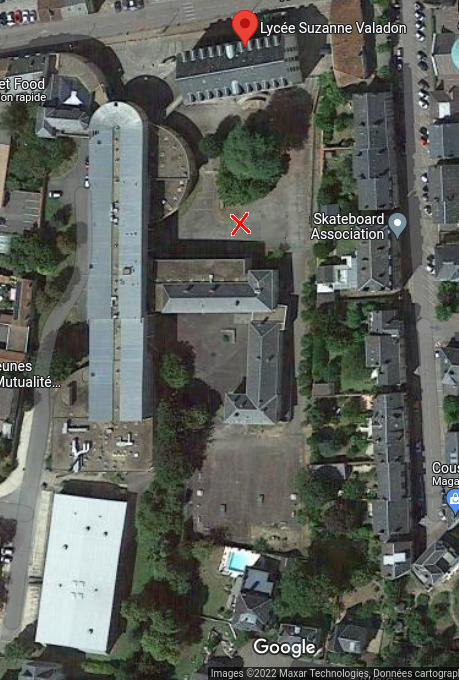
\includegraphics{valadon.png}
\end{figure}
\vfill

\newpage
\section*{L'application SatStat.}
\begin{multicols}{2}
\begin{figure}
	\centering
	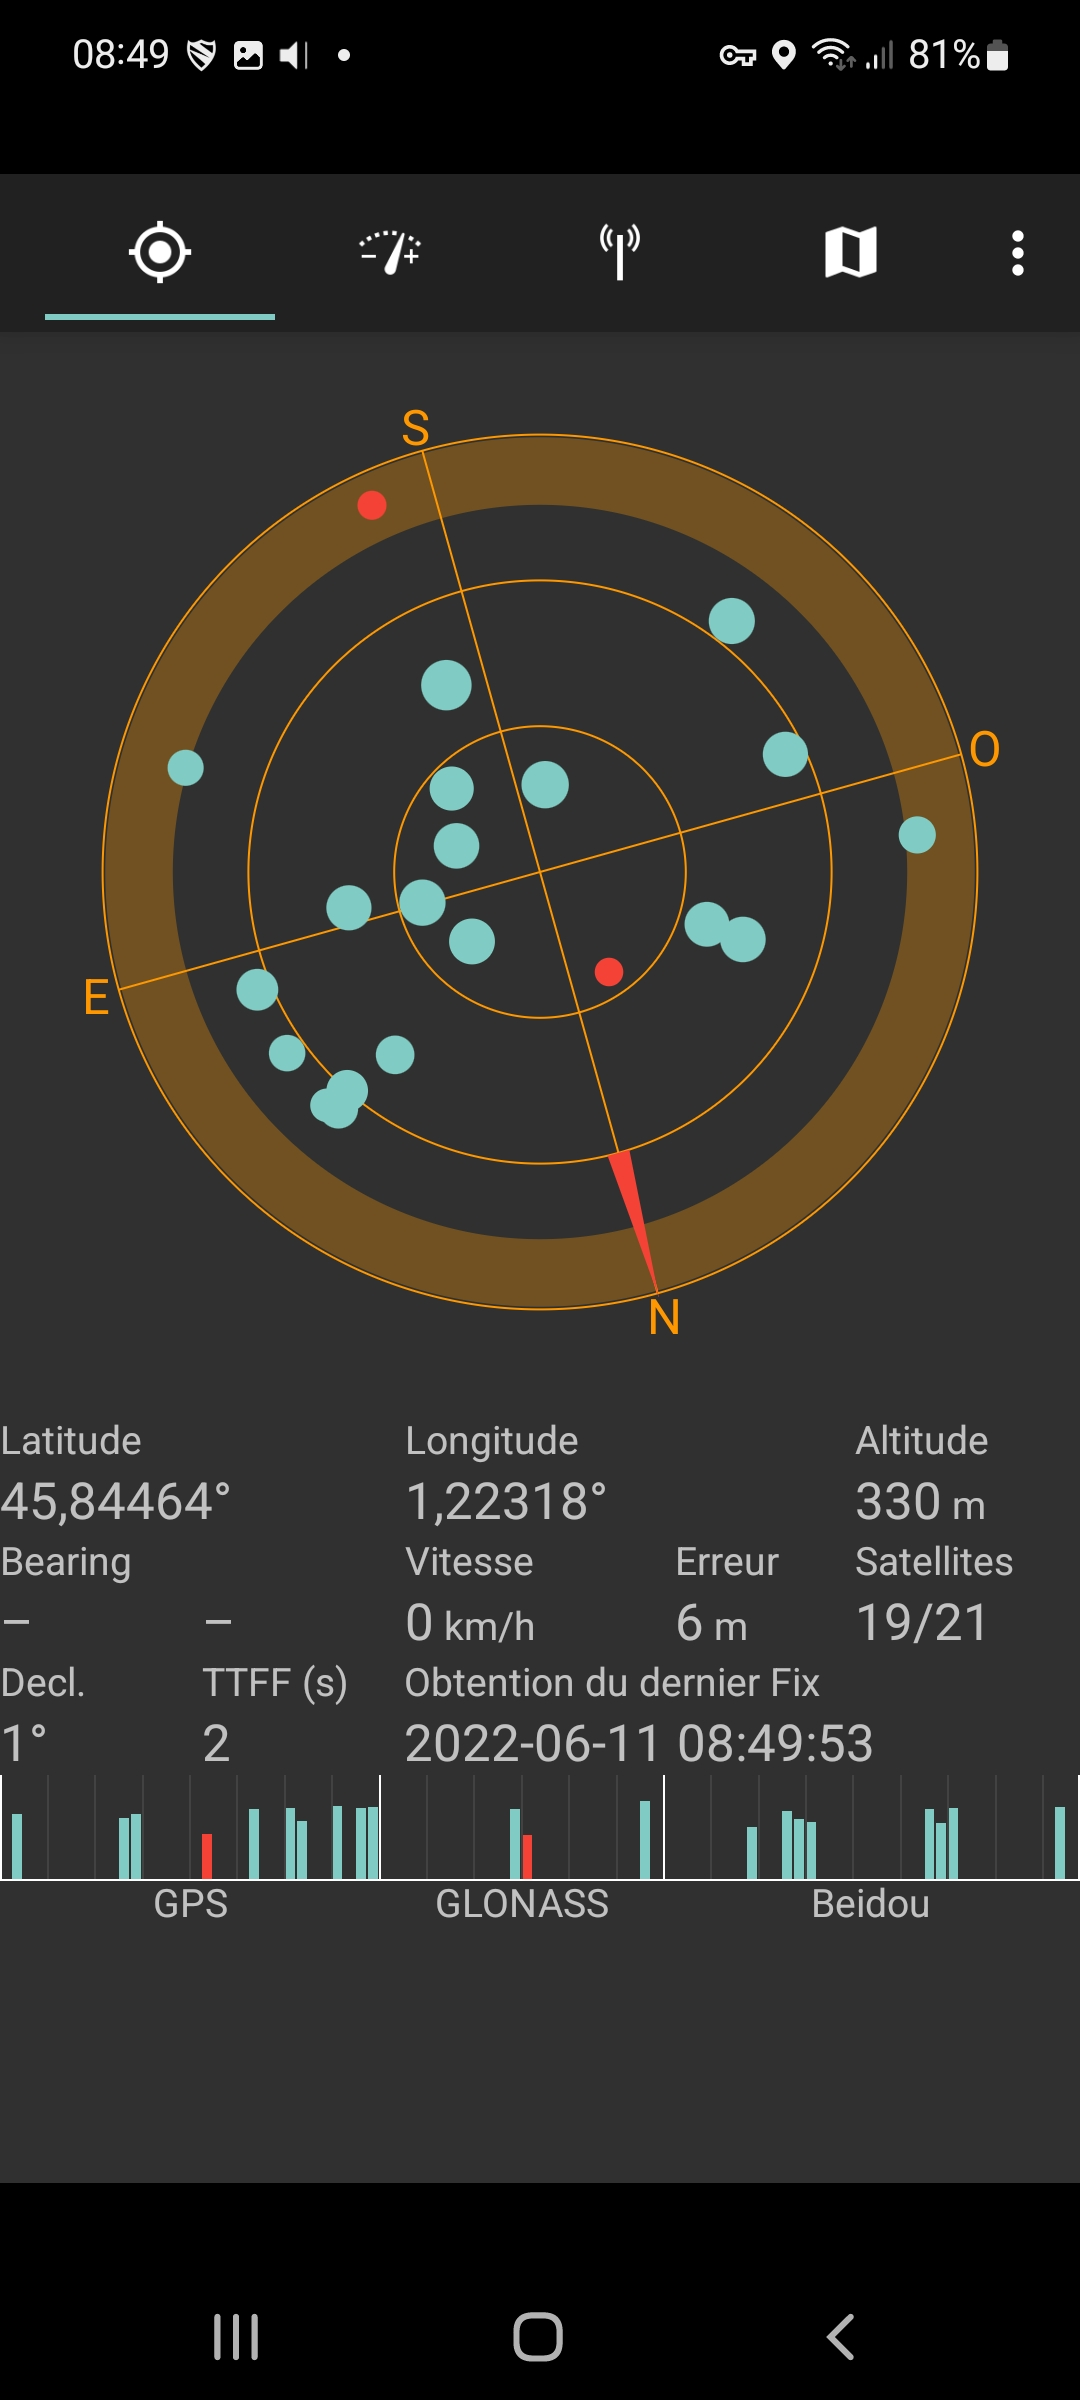
\includegraphics{satstat.jpg}
\end{figure}

\columnbreak

Ci-contre, à gauche, l'application satstat, géolocalise le dispositif et donne des informations en dessous du diagramme circulaire.

Pour pouvoir l'utiliser penser à activer la géolocalisation.

\vspace{2cm}

Effectuez les différentes tâches qui suivent à l'aide de l'application et revenez ensuite en classe.
\end{multicols}

\section{Activité 1.}
Rendez-vous dans la cours et pointez toutes les coordonnées géographiques des extrémités des bâtiments et de la cour. 
Notez-les dans le tableau qui suit. 
\begin{table}
	\centering
	\renewcommand*{\baselinestretch}{1.45}
	\rowcolors{1}{black!5!white}{white}
	\begin{tabular}{| m{0.03\linewidth} | m{0.60\linewidth} | m{0.15\linewidth} | m{0.15\linewidth} |}
		\hline
		n$^0$ & Désignation du point (place le n$^0$ sur la carte) & latitude & longitude \cr
		\hline
		1 &  &  &  \cr
		\hline
		2 &  &  &  \cr
		\hline
		3 &  &  &  \cr
		\hline
		4 &  &  &  \cr
		\hline
		5 &  &  &  \cr
		\hline
		6 &  &  &  \cr
		\hline
		7 &  &  &  \cr
		\hline
		8 &  &  &  \cr
		\hline
		9 &  &  &  \cr
		\hline
		10 &  &  &  \cr
		\hline
	\end{tabular}
\end{table}

\section{Activité 2}
Rendez-vous à la marque rouge, notez les coordonnées du point. 
puis notez les coordonnées des deux points sur le même méridien que celui de la croix positionnés aux extrémités de la cours.
\begin{table}
	\centering
	\rowcolors{1}{white!95!black}{white}
	\begin{tabular}{| m{0.02\linewidth} | m{0.63\linewidth} | m{0.12\linewidth} | m{0.12\linewidth} |}
		\hline
		 & Désignation de la position & latitude & longitude \cr
		\hline
		1 & croix rouge (1) &  &  \cr
		\hline
		2 & même latitude que (1), point le plus occidental &  &  \cr
		\hline
		3 & même latitude que (1), point le plus oriental &  &  \cr
		\hline
		4 & même longitude que (1), point le plus septentrional &  &  \cr
		\hline
		5 & même longitude que (1), point le plus austral &  &  \cr
		\hline
	\end{tabular}
\end{table}

\section{Un peu de calcul.}
\subsection{Conversions décimal - sexagésimal}
Convertissez toutes les coordonnées de la seconde activité en coordonnées sexagésimales (degrés, minutes et secondes). 
\begin{table}
	\centering
	\rowcolors{1}{white!95!black}{white}
	\begin{tabular}{| m{0.02\linewidth} |  m{0.20\linewidth}  m{0.20\linewidth} || m{0.20\linewidth}  m{0.20\linewidth} |}
		\hline
		n$^0$ & lat. (déc) & $\rightarrow$ lat. (dms) & long. (déc.) & $\rightarrow$ long. (dms) \cr
		\hline
		1 &  &  &  &  \cr
		\hline
		2 &  &  &  &  \cr
		\hline
		3 &  &  &  &  \cr
		\hline
		4 &  &  &  &  \cr
		\hline
		5 &  &  &  &  \cr
		\hline
	\end{tabular}
\end{table}

\subsection{Calcul.}
En supposant que le rayon de circonférence de la terre au lycée est R~=~6~400,3~km, calculez la distance entre les extrémités les plus proches de la cour.

\end{document}